\documentclass[border=3pt,tikz]{standalone}

\usepackage{tikz}
\usepackage{fontspec}
\usepackage[T1]{fontenc}
\setmainfont{Source Sans Pro}
\usetikzlibrary{positioning, arrows.meta, decorations.markings,calc}
%\renewcommand{\familydefault}{\sfdefault}

\definecolor{jhnavy}{HTML}{002d72}

\begin{document}
		
	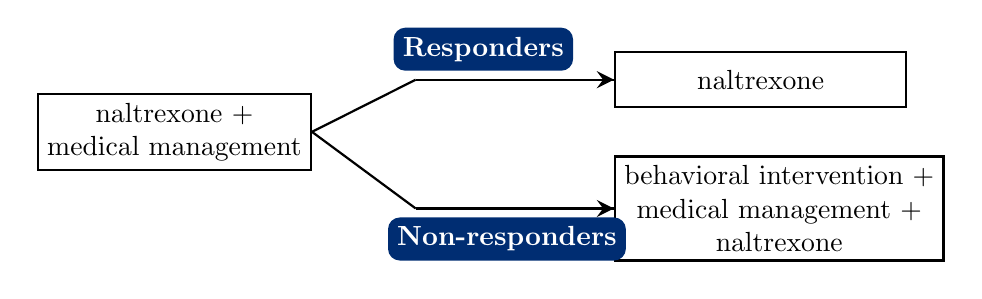
\begin{tikzpicture}[%
		node distance=6mm,
		randomize/.style={
			circle,
			minimum size=6mm,
			thick,
			black,
			draw
		},
		rerand/.style={
			xshift = 15mm
		},
		treatment/.style={
			rectangle,
			minimum size = 7mm,
			thick,
			black,
			anchor=west,
			align=center,
			draw
		},
		stg2tx/.style={
			minimum width= 37mm
		},
		blank/.style={
			rectangle,
			minimum size=2mm
		},
		subgroup/.style={
			rectangle,
			rounded corners=1.5mm,
			thin,
			minimum size=6mm,
			black,
			draw
		},
		rlabel/.style={
%			font=\footnotesize,
			above,
			xshift=-4mm,
			align=left,
			fill=jhnavy,
			text=white,
			rounded corners=1.5mm,
			font=\bfseries
		},
		nrlabel/.style={
%			font=\footnotesize,
			below,
			xshift=-1mm,
			align=left,
			fill=jhnavy,
			text=white,
			rounded corners=1.5mm,
			font=\bfseries
		},
		trialarrow/.style={
			thick,
			decoration={markings,mark=at position 1 with  {\arrow[scale=1.5,>=stealth]{>}}},
			postaction={decorate}
		},
		subsetarrow/.style={
			thin,
			gray,
			dashed,
			decoration={markings,mark=at position 1 with {\arrow[scale=1.2,>=stealth]{>}}},
			postaction={decorate}
		}, thick]
						
		\matrix (dtr) [row sep=-2mm, column sep=12mm]{ %
%			\node [align=center,anchor=west] {\large \textbf{Stage 1}}; & &  \node [align=center,xshift=5mm] {\large \textbf{Stage 2}};\\[5mm]
			
			% DESIGN I
			
			& \node (blank1) [blank] {}; & & \node (stg2R) [treatment,stg2tx] {naltrexone}; \\
			\node (stg1) [treatment] {naltrexone + \\medical management}; & & \\
			& \node (blank2) [blank] {}; & & \node (stg2NR) [treatment,stg2tx] {behavioral intervention + \\ medical management + \\ naltrexone}; \\
		};
	
%		\draw[dashed,lightgray] (time1.north) -- (R2-III.south);
%		\draw[dashed,lightgray] (R2-III.north) -- (R3-II.south);
%		\draw[dashed,lightgray] (R3-II.north) --++(90:3.2cm);
%		
%		\draw[dashed,lightgray] (time2.north west) --++(90:33cm);
	
		% DESIGN I LINES
		
		\draw (stg1.east) -- (blank1.center);
		\draw (stg1.east) -- (blank2.center);
		\draw[trialarrow] (blank1.center) -- node[rlabel, yshift=1mm] {Responders} (stg2R.west);
		\draw[trialarrow] (blank2.center) -- node[nrlabel,yshift=-1mm] {Non-responders} (stg2NR.west);
	
%		\draw[trialarrow] (R1-I) -- (A-I.west);
%		\draw (A-I.east) -- (b1-I.center);
%		\draw (A-I.east) -- (b2-I.center);
%		\draw[trialarrow] (b1-I.center) -- node[rlabel] {Responders} (R2-I.west);
%		\draw[trialarrow] (b2-I.center) -- node[nrlabel] {Non-Responders} (R3-I.west);
%		\draw[trialarrow] (R2-I.east) -- (C-I.west);
%		\draw[trialarrow] (R2-I.east) -- (D-I.west);
%		\draw[trialarrow] (R3-I.east) -- (E-I.west);
%		\draw[trialarrow] (R3-I.east) -- (F-I.west);
%		
%		\draw[trialarrow] (R1-I) -- (B-I.west);
%		\draw (B-I.east) -- (b3-I.center);
%		\draw (B-I.east) -- (b4-I.center);
%		\draw[trialarrow] (b3-I.center) -- node[rlabel] {Responders} (R4-I.west);
%		\draw[trialarrow] (b4-I.center) -- node[nrlabel] {Non-Responders} (R5-I.west);
%		\draw[trialarrow] (R4-I.east) -- (G-I.west);
%		\draw[trialarrow] (R4-I.east) -- (H-I.west);
%		\draw[trialarrow] (R5-I.east) -- (I-I.west);
%		\draw[trialarrow] (R5-I.east) -- (J-I.west);
%		
%		\draw[subsetarrow] (C-I.east) -- (sbgp1.west);
%		\draw[subsetarrow] (D-I.east) -- (sbgp2.west);
%		\draw[subsetarrow] (E-I.east) -- (sbgp3.west);
%		\draw[subsetarrow] (F-I.east) -- (sbgp4.west);
%		\draw[subsetarrow] (G-I.east) -- (sbgp5.west);
%		\draw[subsetarrow] (H-I.east) -- (sbgp6.west);
%		\draw[subsetarrow] (I-I.east) -- (sbgp7.west);
%		\draw[subsetarrow] (J-I.east) -- (sbgp8.west);
		
		% TIME LINES
		
%		\draw (time0) -- (time1) -- (time2);
\end{tikzpicture}
\end{document}